%%%%%%%%%%%%%%%%%%%%%%%%%%%%%%%%%%%%%%%%%%%%%%%%%%%%%%%%%%%%%%%%%%%%%%%%%%%%%%%%
%2345678901234567890123456789012345678901234567890123456789012345678901234567890
%        1         2         3         4         5         6         7         8

\documentclass[letterpaper, 10 pt, conference]{ieeeconf}  % Comment this line out
                                                          % if you need a4paper
%\documentclass[a4paper, 10pt, conference]{ieeeconf}      % Use this line for a4
                                                          % paper

\IEEEoverridecommandlockouts                              % This command is only
                                                          % needed if you want to
                                                          % use the \thanks command
\overrideIEEEmargins
% See the \addtolength command later in the file to balance the column lengths
% on the last page of the document

\usepackage[utf8]{inputenc}
\usepackage[T1]{fontenc}

% The following packages can be found on http:\\www.ctan.org
\usepackage{graphicx} % for pdf, bitmapped graphics files
%\usepackage{epsfig} % for postscript graphics files
%\usepackage{mathptmx} % assumes new font selection scheme installed
%\usepackage{mathptmx} % assumes new font selection scheme installed
%\usepackage{amsmath} % assumes amsmath package installed
%\usepackage{amssymb}  % assumes amsmath package installed

\title{\LARGE \bf
OTH-Wiki
}

%\author{ \parbox{3 in}{\centering Huibert Kwakernaak*
%         \thanks{*Use the $\backslash$thanks command to put information here}\\
%         Faculty of Electrical Engineering, Mathematics and Computer Science\\
%         University of Twente\\
%         7500 AE Enschede, The Netherlands\\
%         {\tt\small h.kwakernaak@autsubmit.com}}
%         \hspace*{ 0.5 in}
%         \parbox{3 in}{ \centering Pradeep Misra**
%         \thanks{**The footnote marks may be inserted manually}\\
%        Department of Electrical Engineering \\
%         Wright State University\\
%         Dayton, OH 45435, USA\\
%         {\tt\small pmisra@cs.wright.edu}}
%}

\author{Dominik Smrekar, Johannes Horst, Patrick Sabau, Saniye Ogul und Tobias Schotter}% <-this % stops a space



\begin{document}



\maketitle
\thispagestyle{empty}
\pagestyle{empty}

\section{EINLEITUNG}

Ziel dieses Projektes ist es, eine Web-Anwendung zu entwickeln, die dem Nutzer dabei helfen soll, leichter an relevante Informationen der Technischen Hochschule Amberg-Weiden zu kommen. Da die offizielle Hochschulseite für neue und alte Studenten unübersichtlich ist, gehen viele signifikante Informationen unter. Manche finden die Links zu den Online-Portalen nicht und andere werden mit Informationen bombardiert. Dies führte zur Idee eine Webseite für die OTH-AW zu erstellen, indem Informationen einfach und strukturiert für Studierende von Studierenden angesammelt werden.

%Die Oberfläche der Web-Anwendung orientiert sich an Wikipedia, da dies eine der meist verwendeten Informationsquellen im Internet ist. Die Struktur ist deshalb weit geläufig. Dadurch entsteht der Vorteil, dass sich das Nutzererlebnis der Anwendung steigert und Nutzer nicht desorientiert sind. Zudem wird die gesamte Anwendung durch eine Datenbank gestützt und unterstützt, um Nutzerfunktionalitäten gewährleisten zu können.


\section{VERWANDTE ARBEITEN}

Als primäre Inspiration dient die freie Enzyklopädie Wikipedia, da sie eine übersichtliche und saubere Möglichkeit der Informationsdarstellung bietet. Hierbei sind das Design und die Struktur höchst vertraut, da jeder schon in irgendeiner Form mit Wikipedia in Kontakt getreten ist.

Darüber hinaus inspiriert uns die Software Confluence, aufgrund der Wikipedia artigen Strukturierung von Nutzer priorisierten Informationen.

Abschließend ist die Internetseite der Hochschule Amberg-Weiden selbst zu erwähnen, da sie unter anderem Informationen für Studierende bereitstellt. Jedoch zeigen sich Schwächen bzw. fehlende Möglichkeiten der Informationsbereitstellung von Studierenden für Studierende.



\section{ANFORDERUNGEN}

Grundlegend lassen sich die Ziele der Projektarbeit in 5 Abschnitte untergliedern. Hierzu gehört das Frontend (A), Backend + Datenbank (B) und das Deployment (C). Weitere optionale Features sind ebenfalls unter den entsprechenden Punkten zu finden, jedoch sind einige dieser auch in einem separaten Unterpunkt (D) aufgelistet. Die Anforderungen werden durch den Punkt Testabdeckung (E) abgerundet.

Zur Identifikation von Anforderungen werden zuerst die User Stories für die Projektarbeit betrachtet.

Das führt zum Ziel, das Projekt ausführlich anzupassen und den Integrationsaufwand so gering wie möglich zu halten. Für die Anforderungen wurden die Sicht und die Wünsche des Benutzers in Bezug auf OTH-Wiki beschrieben. 

\subsection{Frontend} 

Als Nutzer möchte ich, dass mir die Texte der Artikel angezeigt werden, um aus ihnen die gewollten Informationen entnehmen zu können.

Als Nutzer möchte ich neue Texte schreiben, oder bestehende Texte bearbeiten können, um fehlende Infos hinzuzufügen oder falsche Aussagen nachbessern zu können.
\begin{itemize}
\item Beim Betätigen des „Edit-Buttons“ gibt es ein Freitextfeld zum Bearbeiten des Textes
\end{itemize}

Als Nutzer möchte ich mithilfe der Suche passende Artikel finden, wodurch Zeit des selber Suchens gespart wird .
\begin{itemize}
\item Schlüsselwörter Suche
\end{itemize}


\begin{figure}[thpb]
      \centering
      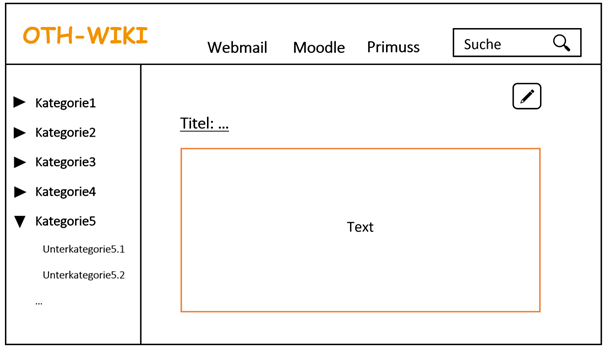
\includegraphics[scale=0.55]{abbildungen/frontend.png}
      \caption{Konzeptzeichnung Frontend}
      \label{fig:frontend}
 \end{figure}
 
Abbildung \ref{fig:frontend} zeigt eine Konzeptzeichnung des Frontends. Diverse Features sind in diesem zu erkennen:
\begin{itemize}
\item Kategorien sind aufklappbar
\item Webmail, Moodle und Primuss sind Links
\item Durch Suche können Artikel mit Schlüsselwörtern gesucht werden
\item Titel und Text werden dynamisch angezeigt
\item Texte können bearbeitet werden, durch „Edit-Button“
\end{itemize}

\subsection{Backend + Datenbank}

Als Entwickler möchte ich eine Datenbank, welche nur vom Backend (welches eine REST-API bereit stellt) angesprochen werden kann. Folgende Features sind gefordert:

\begin{itemize}
\item Es soll die Möglichkeit bestehen, Texte als Website-Inhalt zu schreiben (Markdown Formatierung)
\item Artikel sollen aus der Datenbank über die REST-API abrufbar sein
\item Geänderte Artikel sollen in der Datenbank gespeichert und zusätzlich versioniert werden.
\item Es soll eine hierarchische Suche geben, welche in der Datenbank nach Keywords in Texten oder Tags etc. sucht.
\item \textit{Optional:} Weiter ist es möglich, die Artikel mit entsprechenden Bildern zu ergänzen
\item \textit{Optional:} Eine Kommentarfunktion erlaubt Nutzern das Hinzufügen von Kommentaren und/oder Fragen zu speziellen Inhalten.

\end{itemize}

\subsection{Deployment}
Jede der Teilkomponenten wird in einem eigenen Docker Container gepackt. Mittels docker-compose können diese Container gleichzeitig gestartet und gemanaget werden.
\begin{itemize}
\item \textit{Optional:} Der Container werden zusätzlich in einen Kubernetes-Cluster deployed
\end{itemize}

\subsection{optionale Ziele}
\begin{itemize}
\item \textit{Optional:} Nutzer haben die Möglichkeit, Fragen an alle aktiven Nutzer zu stellen. Entweder über einen eigenen Fragen-Artikel oder einen dafür spezialisierten Abschnitt der Seite.
\item \textit{Optional:} Nutzern wird angeboten, Bilder/Dateien auf der Plattform auszutauschen/hochzuladen.
\end{itemize}

\subsection{Testabdeckung}
Als Entwickler möchte ich eine ausreichende Testabdeckung, damit Fehler frühzeitig erkannt werden. Akzeptanzkriterien sind:
\begin{itemize}
\item Die Code-Qualität jeder Komponente wird durch Unit-Tests gewährleistet
\item Die Code-Coverage liegt bei mindestens 50\%.
\end{itemize}


\section{ARCHITEKTUR}

Teile der Architektur wurden bereits in Abschnitt II. erwähnt, jedoch werden diese nochmal detaillierter spezifiziert.

\subsection{Frontend}
Das Frontend wird mittels des Framework \textbf{Angular} entwickelt. Dieses setzt auf NodeJS sowie auf die Programmiersprache TypeScript, welche JavaScript um statischen Datentypen ergänzt. 
Angular kann über einen speziellen \textit{build}-Befehl eine einzelne \textbf{.html} Seite generieren, welche anschließend mittels eines Http-Servers geserved werden kann. Diese Aufgabe übernimmt \textbf{nginx}.
Der zugehörige Docker-Container besteht dabei aus zwei Teilen, einem Build-Container und einem Application-Container. Diese beiden übernehmen dabei den  \textbf{Build} und den \textbf{Serving} Schritt.

\textbf{Nginx} hat neben dem Serving der .html-Seite noch zwei zusätzliche Aufgaben: 
\begin{itemize}
\item SSL-Verschlüsselung mittels Zertifikate von \textbf{Let's Encrypt}
\item Proxy für die Backend-Applikation zur Vermeidung von CORS-Fehlern
\end{itemize}

\subsection{Backend}
Das Backend wird mittels FastAPI und Python umgesetzt.
Die Hauptaufgabe des Backends besteht es darin, das Datenmodell aus Abbildung \ref{fig:db} in einer MongoDB Datenbank zu verwalten. 
\begin{figure}[thpb]
      \centering
      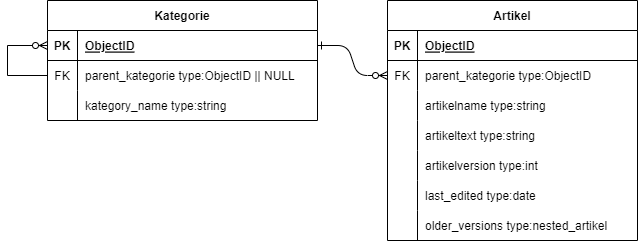
\includegraphics[scale=0.35]{abbildungen/db.drawio.png}
      \caption{Datenmodell}
      \label{fig:db}
 \end{figure}
 
Kategorien dienen zur Gruppierung der einzelnen Artikel und können auch ineinander verschachtelt werden. Jeder Artikel ist einer Kategorie zugeordnet und enthält dabei die Daten, welche den Artikel ausmachen (in Abbildung \ref{fig:db} ist nur ein kleiner Teil der Inhalte dargestellt).
 
Das Backend nutzt REST für die Kommunikation mit dem User. Die wichtigsten Endpoints sind dabei:
\begin{itemize}
\item \textit{GET} /kategorie
\item \textit{GET} /artikel/<id>/<version>
\item \textit{POST} /artikel 
\end{itemize}

Die beiden \textbf{GET} Endpoints dienen dabei der Informationsdarstellung im Frontend, wohingegen der \textit{POST} (oder auch \textbf{PUT}) Endpoint entsprechende Änderungen in der Datenbank persistiert.

\subsection{docker-compose}
Docker-compose bietet eine Möglichkeit, mehrere Docker Container zu managen und diese gleichzeitig zu starten. Entsprechend werden die einzelnen Teilkomponenten mit diesem Tool orchestriert.


\subsection{Interaktion des Users}
Abbildung \ref{fig:arch} zeigt, wie ein User mit der Anwendung interagiert.

\begin{figure}[thpb]
      \centering
      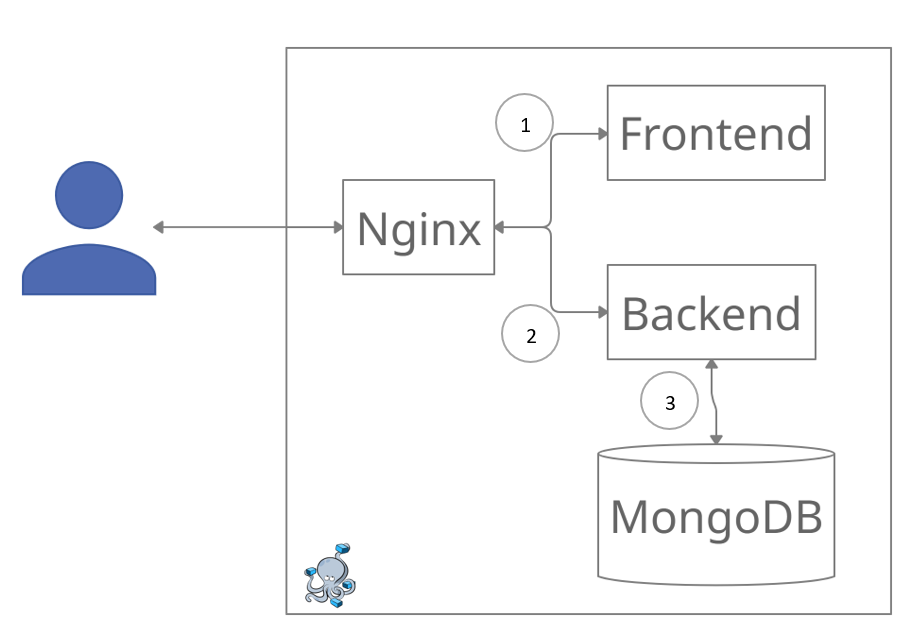
\includegraphics[scale=0.35]{abbildungen/architektur.PNG}
      \caption{Konzept Architektur}
      \label{fig:arch}
 \end{figure}

Der User erhält mittels einer GET-Anfrage das Frontend von dem nginx-Server (Schritt 1). Standardmäßig werden Inhalte von Angular Seiten clientseitig angefragt. Dies bedeutet, es erfolgen weitere REST-Calls des Users (über JavaScript Code der Website) über den nginx-Proxy an den Backend-Service (Schritt 2). Dieser Service, ist die einzige Verbindung zur Datenbank. Nach Verarbeitung der Anfrage (Schritt 3), wird eine entsprechende Antwort (z.B. mit dem Inhalt des Artikel) an den User zurückgesendet.

%%%%%%%%%%%%%%%%%%%%%%%%%%%%%%%%%%%%%%%%%%%%%%%%%%%%%%%%%%%%%%%%%%%%%%%%%%%%%%%%%%%%%%%%%%%%%%
\addtolength{\textheight}{-10cm}   % This command serves to balance the column lengths
                                  % on the last page of the document manually. It shortens
                                  % the textheight of the last page by a suitable amount.
                                  % This command does not take effect until the next page
                                  % so it should come on the page before the last. Make
                                  % sure that you do not shorten the textheight too much.
%%%%%%%%%%%%%%%%%%%%%%%%%%%%%%%%%%%%%%%%%%%%%%%%%%%%%%%%%%%%%%%%%%%%%%%%%%%%%%%%%%%%%%%%%%%%%%

\end{document}
